%!TEX root = ULL_thesis_template.tex 
\chapter{Mechanical Design of a the Monopode Jumping System}
\label{chapter4}

Often it is the goal of a controls engineer to design a controller to accommodate and manipulate systems according to the system description provided. However, research has been conducted showing the value of studying the manipulation of mechanical design parameters in order to achieve a desired system behavior \cite{Li2001}. In this chapter, reinforcement learning is shown to be useful as a tool to learn mechanical designs given a predefined system controller for the monopode jumping system. RL has been shown to be an effective strategy for finding optimal concurrent designs for many different types of systems \cite{Schaff2019e, Luck2019, Ha2019j}. It has even shown its ability to define designs that are successfully deployed on physical hardware \cite{Chen2020}. It is comparable to work where evolutionary algorithms are deployed to optimize physical parameters of systems for improved energy efficiency \cite{Wang2019, Hu2020}. Here, RL is used to define an optimal design for the monopode jumping system described in Chapter~\ref{chapter2}.

\section{Learning a Mechanical Design}
Section~\ref{sec:rl} describes the common deployment methodology of an RL problem where defining a control policy for a robotic system is often the primary goal. In this chapter, rather than finding a control policy for a defined robotic system, RL is deployed to find a mechanical design for a defined control input. To do this, the general methods in setting up the problem have to change. Figure~\ref{fig:TD3_mech_design} shows the general flow of information for the algorithm.

% 
\begin{figure}[tb!]
        \centering
        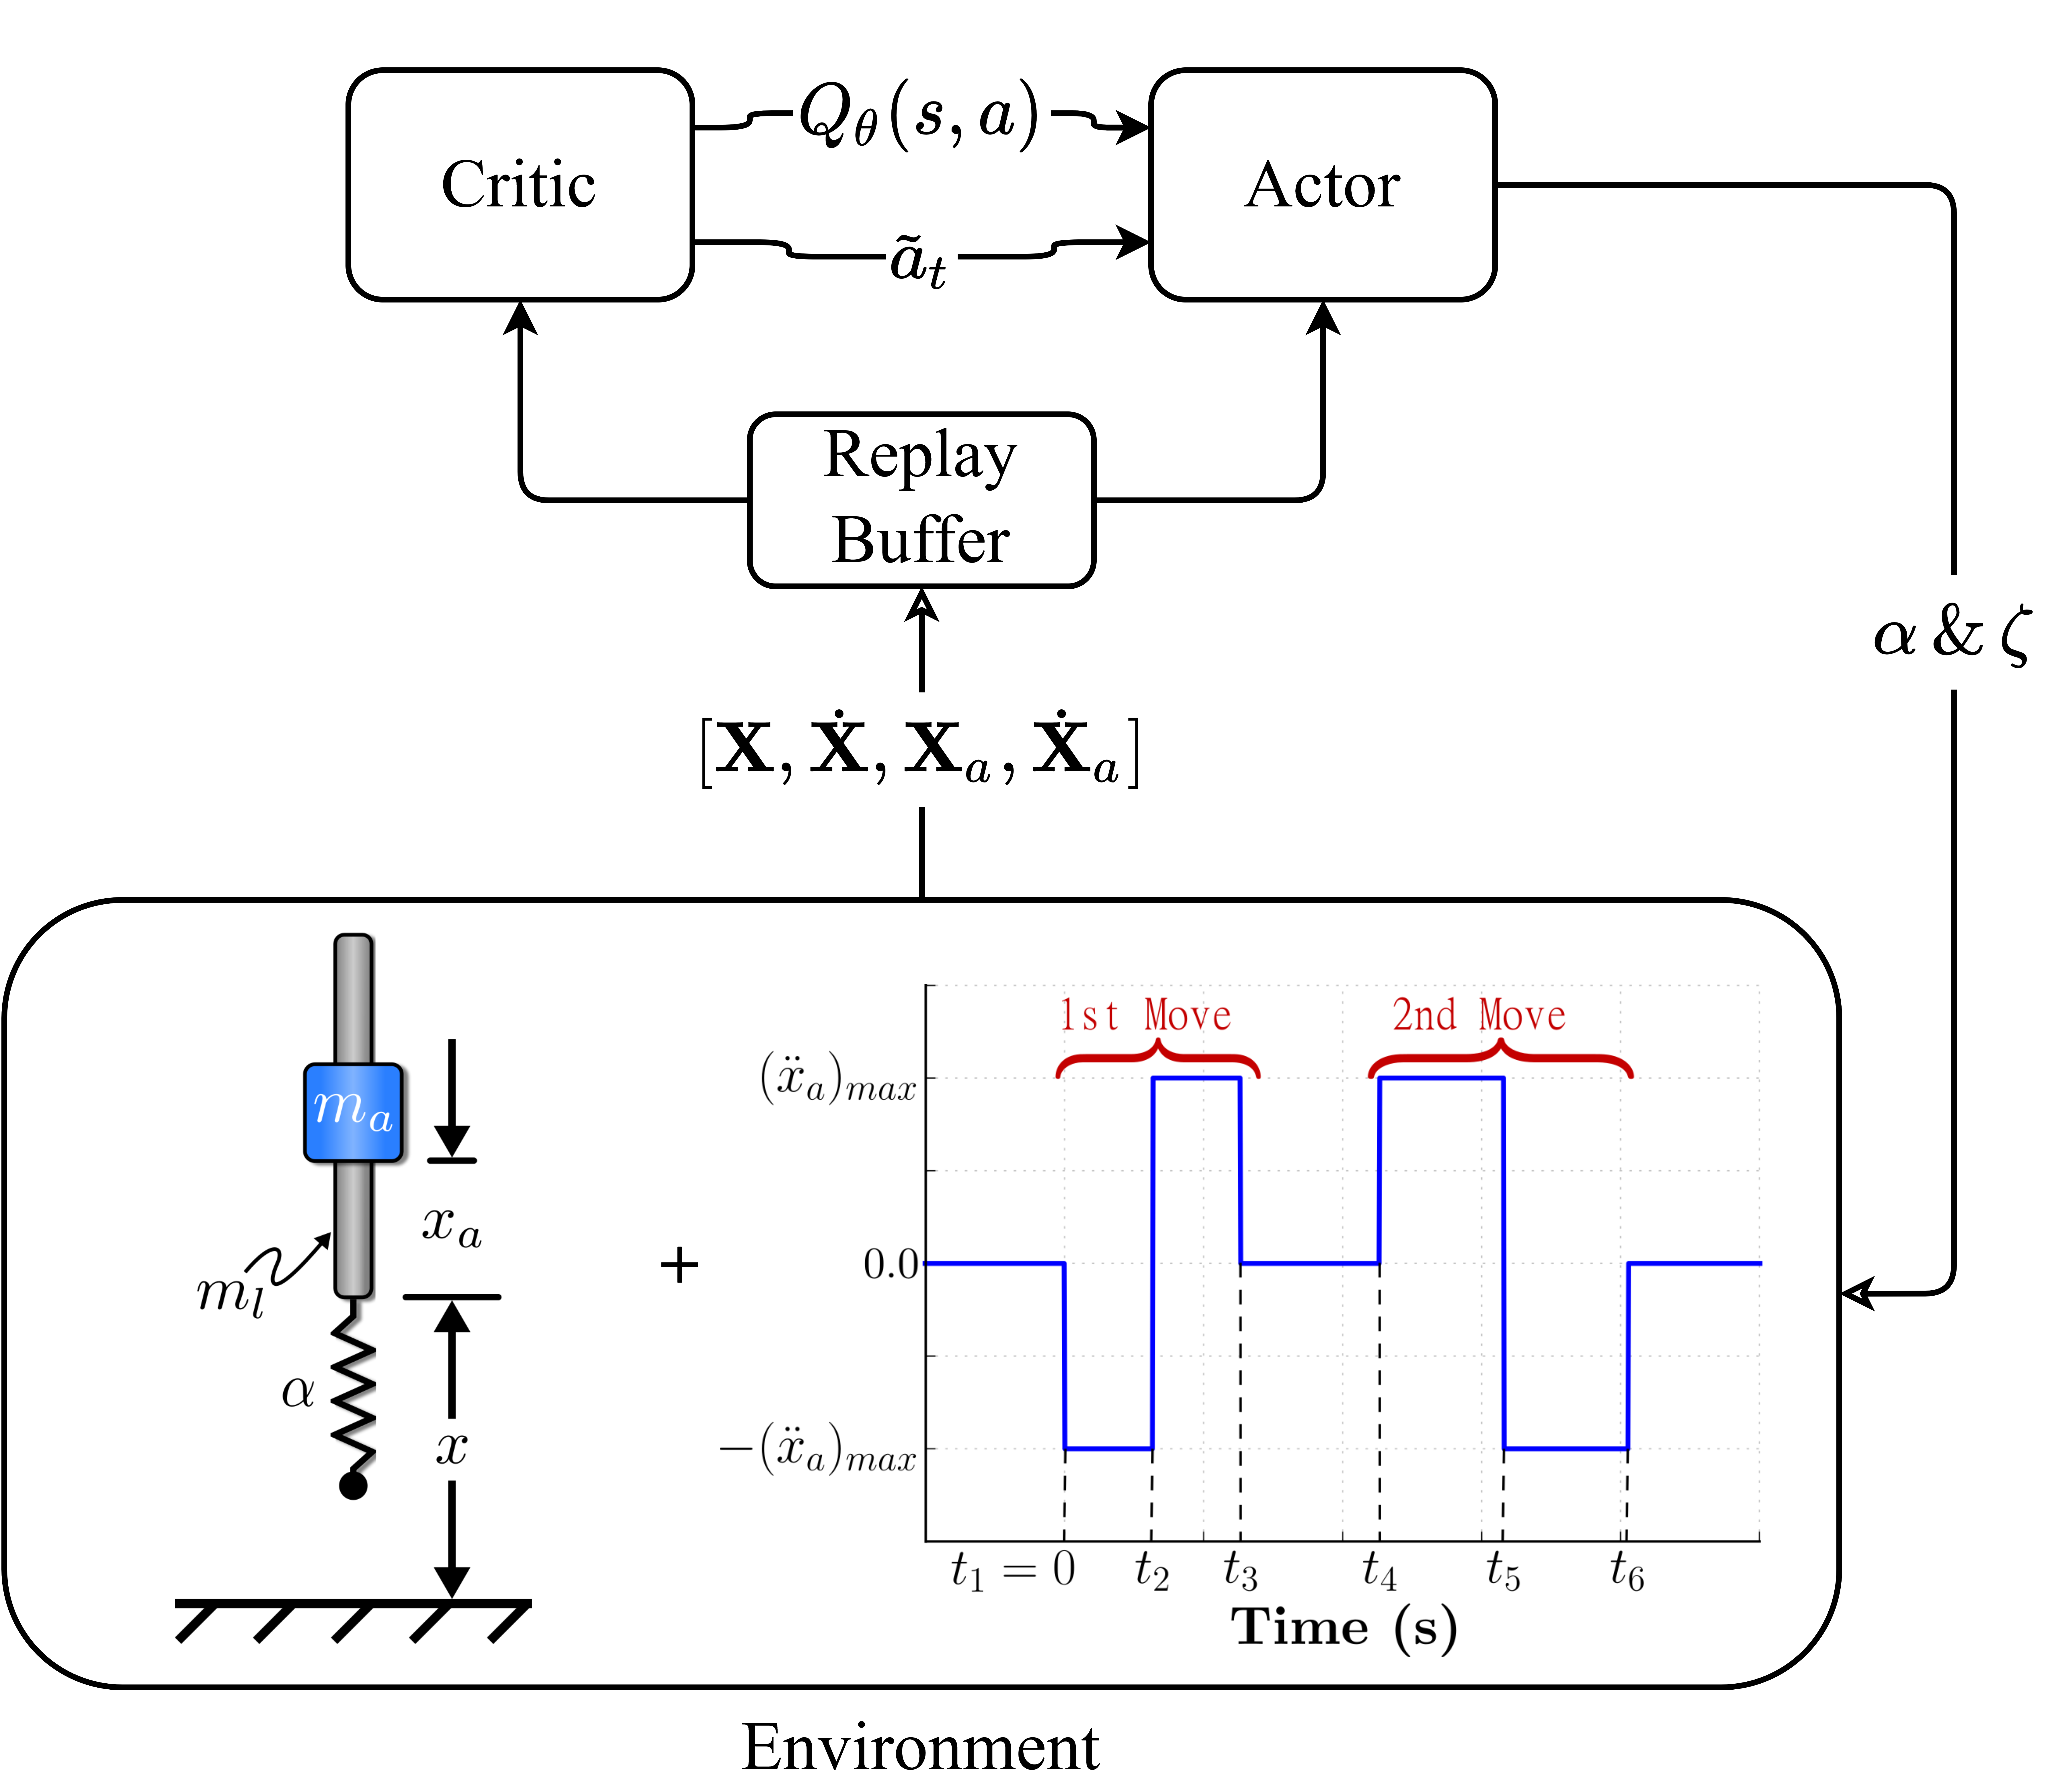
\includegraphics[width=0.95\textwidth]{figures/Ch4/TD3_Mech_Params.drawio.png}  
        \caption{Learning a Mechanical Design}
        \label{fig:TD3_mech_design}
\end{figure}
% 

The RL problem is similar to the common use case in that the algorithm utilizes the same information types to optimize a design, such as the state of the environment and the reward. The interaction of the algorithm with the environment is drastically different, however. The action space, instead of being a command type input, is a range of design choices for a set of parameters within a simulation of a system. Applying these actions within the environment, rather than changing the state of a robotic system from state $s$ to $s'$, instead simulates a system within the environment from time $t=0$ to time $T$ using a predefined control input. Because of this, the state saved as a transition is a matrix of states rather than a single vector state. The reward does not differ greatly in that it is based on the state of the system. The difference is that the information stored in a single state transition is much greater so the reward can be defined to utilize all the information.

For the work presented in this chapter, the predefined control input used to simulate the monopode system within the environment at each step was an optimized controller generated using the input shaping techniques discussed in Section~\ref{sec:controller_input} as is shown in Figure~\ref{fig:TD3_mech_design}. Having been shown to be a useful technique for generating optimal control strategies, it was of interest to evaluate if an optimal mechanical design could be found to accompany the input.

\section{Environment Definition}
To allow the agent to find a mechanical design, a reinforcement learning environment conforming to the OpenAI Gym standard \cite{Brockman2016c} was created. The monopode model described in Chapter~\ref{chapter2} was used as the simulation, and the fixed controller input was based on the work described in Section~\ref{sec:controller_input}. The mechanical parameters the agent was tasked with optimizing were the spring constant and the damping ratio of the monopode system. At each episode during training, the policy of the algorithm selected a set of design parameters from a distribution of predefined parameter ranges and saved the timeseries simulation information in the replay buffer. The actions applied, $\mathcal{A}$, within the environment were the designs selected and were defined as follows:
% 
\begin{equation}
    \label{eq:mech_action}
    \begin{aligned}
    \mathcal{A} = \{ \{ a_{\alpha} \in \mathbb{R}: [0.1 \alpha_{nom}, 1.9 \alpha_{nom}] \}, \, \{ a_{\zeta} \in \mathbb{R}: [0.1 \zeta_{nom}, 1.9 \zeta_{nom}] \} \}
    \end{aligned}
\end{equation}
% 
where $\alpha_{nom}$ and $\zeta_{nom}$ are the nominal spring constant and damping ratio of the monopode, respectively; $x_t$ and $\dot{x}_t$ are the rod height and velocity steps of the monopode, and $x_{a_t}$ and $\dot{x}_{a_t}$ are the actuator position and velocity steps of the monopode, all captured during simulation. The action space was set to $\pm$90\% of the nominal values as that percentage allowed for a large variance in performance across the range of designs. The observations saved, were the timeseries information, and were defined as:
% 
\begin{equation}
    \label{eq:mech_transitions}
    \mathcal{S}= \{ \textup{\textbf{X}}, \dot{\textup{\textbf{X}}}, \textup{\textbf{X}}_a, \dot{\textup{\textbf{X}}}_a \}
\end{equation}
% 
where $\textup{\textbf{X}}$, $\dot{\textup{\textbf{X}}}$, $\textup{\textbf{X}}_a$ and $\dot{\textup{\textbf{X}}}_a$ are timeseries data for the position and velocity of the rod, and the position and velocity of the actuator, respectively.


\section{Rewards for Learning Designs}
The RL algorithm was utilized to find designs for two different reward cases. Time series data was captured during the simulation phase of training and was used to evaluate the designs performance through these rewards. The first reward case used was:
%
\begin{equation}
        R_1 = \left \{ \textup{\textbf{X}} \right \}_{\textup{max}}
\end{equation}
% 
where $x_t$ was the rod height of the monopode at each step during simulation. The goal of the first reward was to find a design that would cause the monopode to jump as high as possible. 

The reward for the second case was:
%
\begin{equation}
        R_2 = \frac{1}{\frac{\left | \mathbb{R}_1 - x_s \right |}{x_s} + 1}
\end{equation}
%
where $x_s$ was the desired jump height, which was set to 0.1~m. The second case was utilized to test ability of RL to find a design that minimized the error between the maximum height reached and the desired maximum height to reach.

\section{Design Space Variations}
% 
\begin{figure}[tb!]
        \centering
        \begin{subfigure}{0.75\textwidth}
        \centering
        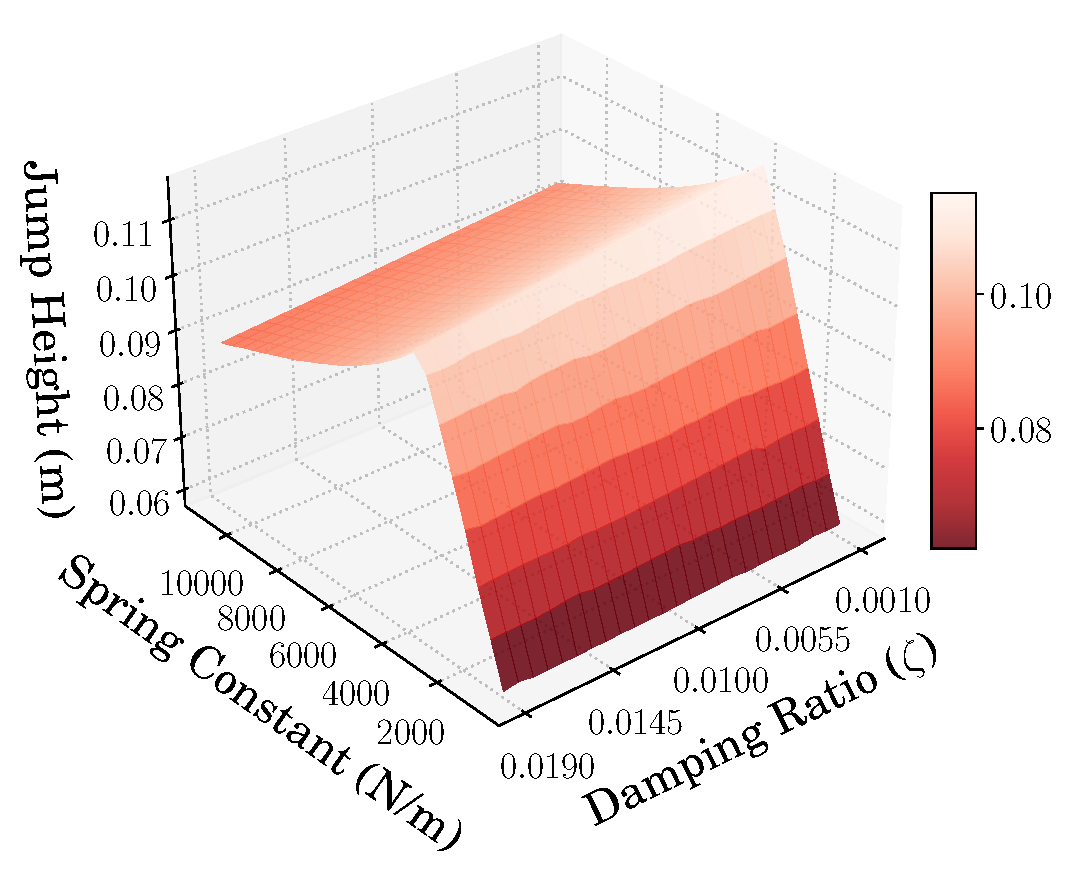
\includegraphics[width=\linewidth]{figures/Ch4/design_space_narr/Design_3D_Plot_0.01_.pdf}
        \caption{Jumping Performance of Narrow Design Space}
        \label{fig:spring_zeta_narr}
        \end{subfigure} \\
        \begin{subfigure}{0.75\textwidth}
        \centering
        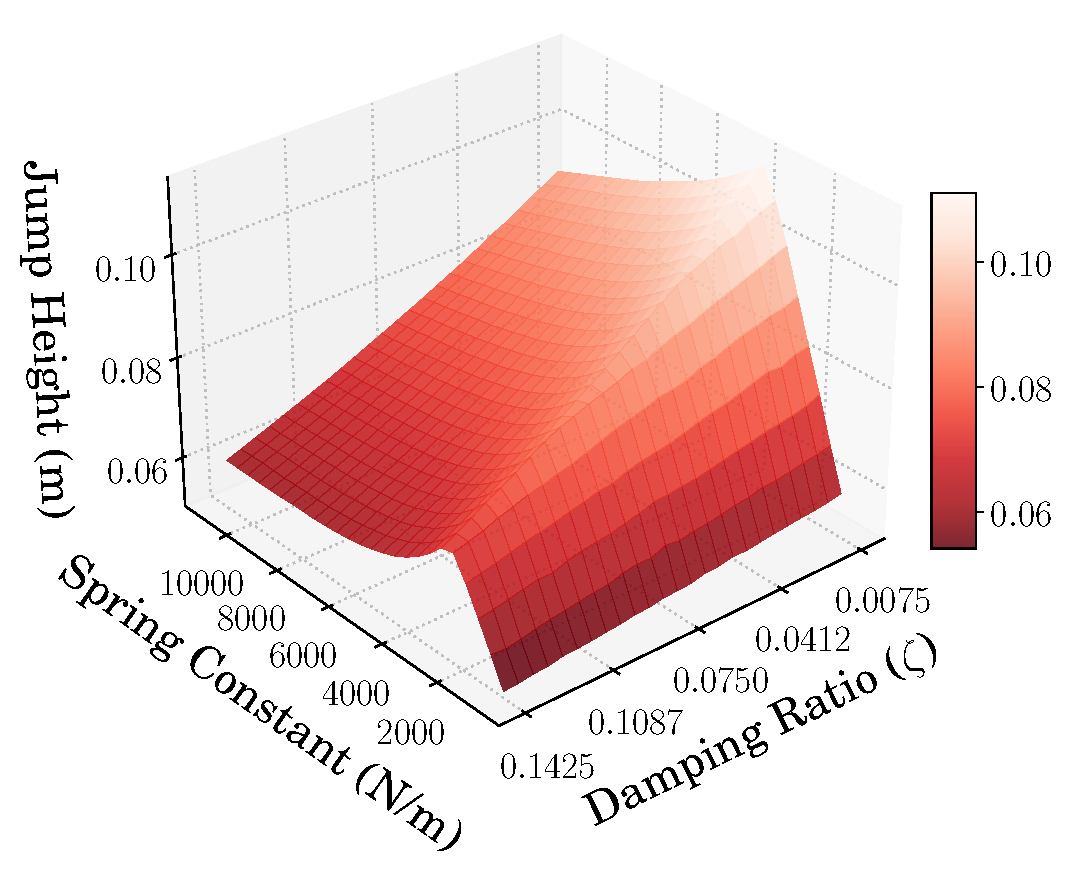
\includegraphics[width=\linewidth]{figures/Ch4/design_space_wide/Design_3D_Plot_0.075_.pdf}
        \caption{Jumping Performance of Wide Design Space}
        \label{fig:spring_zeta_wide}
        \end{subfigure} 
         \caption{Reference Jumping Performance of the Monopode}
         \label{fig:spring_vs_zeta}
\end{figure}

Figure~\ref{fig:spring_vs_zeta} represents the heights the monopode could reach for two different design spaces. The design space provided for the first case, shown in Figure~\ref{fig:spring_zeta_narr}, represents a space where the nominal damping ratio, $\zeta_{nom}$, is $0.01$, such that $\pm0.9 \, \zeta_{nom}$ creates a more narrow design space. This design space also has more values closer to the optimal value therefore making it more difficult to optimize quickly. The design space provided for the second case, shown in Figure~\ref{fig:spring_zeta_wide}, represents a space where the nominal damping ratio, $\zeta_{nom}$, is $0.075$, such that $\pm0.9 \, \zeta$ creates a wider design space. Additionally, there is a more obvious maximum within the design space, making it easer to ascend towards an optimal design. In both cases there are many values that would satisfy the specified height jumping strategy.

\section{Deploying TD3}
% 
\begin{table}[tb!]
\caption{TD3 Training Hyperparameters}
\begin{center}
\vspace{-12pt}
\begin{tabular}{c c}
\textbf{Hyperameter}            & \textbf{Value}                  \\
\hline
\hline
Learning Rate, $\alpha$         & 0.001                           \\
Learning Starts                 & 100 Steps                       \\
Batch Size                      & 100 Transitions                 \\
Tau, $\tau$                     & 0.005                           \\
Gamma, $\gamma$                 & 0.99                            \\
Training Frequency              & 1:Episode                       \\
Gradient Steps                  & $\propto$ Training Frequency    \\
Action Noise,  $\epsilon$       & None                            \\
Policy Delay                    & 1 : 2 Q-Function Updates        \\
Target Policy Noise, $\epsilon$ & 0.2                             \\
Target Policy Clip, $c$         & 0.5                             \\
Seed                            & 100 Random Seeds                \\
\hline
\hline
\end{tabular}
\label{tab:mech_hyperparams}
\end{center}
\end{table}
%
% \begin{figure}[tb!]
%         \centering
%         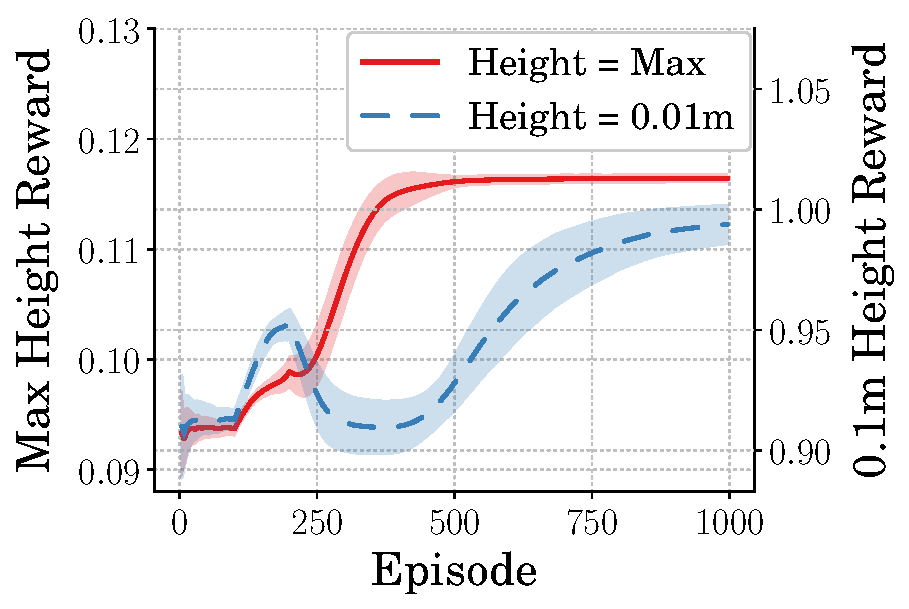
\includegraphics[width=0.75\textwidth]{figures/Ch4/design_space_wide/RewVsTime_2021-10-12_144814.pdf}  
%         \caption{Reward Received During Training}
%         \label{fig:rew_vs_step_narr}
% \end{figure}
% %
% \begin{figure}[tb!]
%         \centering
%         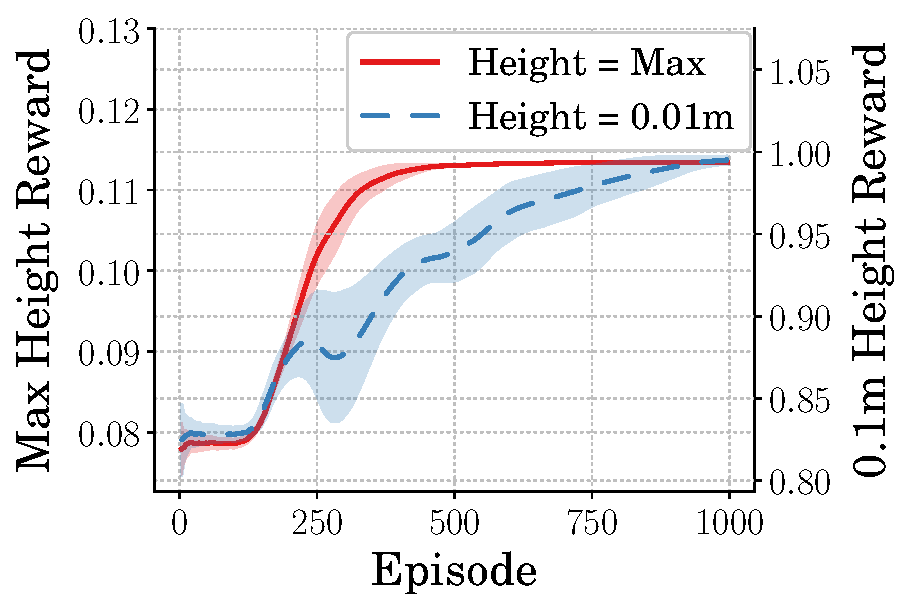
\includegraphics[width=0.75\textwidth]{figures//Ch4/design_space_narr/RewVsTime_2021-10-12_145004.pdf}  
%         \caption{Reward Received During Training}
%         \label{fig:rew_v_step_wide}
% \end{figure}   

The training hyperparameters were selected based on the author of TD3 recommendations and \textbf{StableBaselines3} \cite{stable-baselines3} experimental findings and are displayed in Table~\ref{tab:mech_hyperparams}. All of the hyperparameters, with the exception of the rollout (Learning Starts) and the replay buffer, were set according to \textbf{StableBaselines3} standards. The rollout setting was defined such that the agent could search the design space at random, filling the replay buffer with enough experience to prevent the agent from converging to a design space that was not optimal. The replay buffer was sized proportional to the number of training steps due to system memory constraints. 

%
\begin{figure}[tb!]
        \centering
        \begin{subfigure}{.49\textwidth}
          \centering
          \includegraphics[width=\linewidth]{figures/Ch4/design_space_narr/RewVsTime.png}
          \caption{Reward vs. Episode: Narrow Design Space}
          \label{fig:rew_vs_step_narr}
        \end{subfigure}%
        \hfill
        \begin{subfigure}{.49\textwidth}
          \centering
          \includegraphics[width=\linewidth]{figures/Ch4/design_space_wide/RewVsTime.png}
           \caption{Reward vs. Episode: Wide Design Space}
           \label{fig:rew_v_step_wide}
        \end{subfigure}
         \caption{Reward vs. Episode for Learning Mechanical Design}
         \label{fig:rew_vs_step}
\end{figure}
%    

The average rewards for both the narrow and the wide design space agents are shown in Figure~\ref{fig:rew_vs_step}. They represent the agents learning a converging solution to the problem of finding optimal design parameters. Looking at Figure~\ref{fig:rew_vs_step_narr}, it is apparent that given a more narrow design space, both the high and the specified jumping agents were still able to learn a converging solution. There also exists more variance for the specified-height agent type compared to the agents assigned with maximizing jump height. Looking at Figure~\ref{fig:rew_v_step_wide}, it is apparent that the agents given a wider design space where both able to learn a converging design solution. Though, given more designs to choose from, it appears the specified height agents are taking longer to converge. Additionally, once converged, because there are less values that allow the controller/design architecture to accomplish the tasks, there is less variance seen in the learned designs.

\section{Jumping Performance}
\subsection{Narrow design space}

Figure~\ref{fig:height_v_step_narr} shows the height achieved by the learned designs for the agents given the narrow range of possible damping ratio values. For the agents learning designs to maximize jump height, Figure~\ref{fig:height_v_step_narr} can be compared with Figure~\ref{fig:spring_zeta_narr} showing that the agent learned a design nearing one which would achieve maximum performance. Additionally, looking at the agents learning designs to jump to the specified 0.1~m, the learned designs accomplish this with slightly more variance than that of the maximum height case.
% 
\begin{figure}[tb!]
        \centering
        \includegraphics[width=0.75\textwidth]{figures/Ch4/design_space_narr/HeightVsTime.png}  
        \caption{Height Reached During Training Given Narrow Design Space}
        \label{fig:height_v_step_narr}
\end{figure}
% 

%  
\begin{figure}[tb!]
        \centering
        \begin{subfigure}{.49\textwidth}
                \centering
                \includegraphics[width=\textwidth]{figures/Ch4/design_space_narr/SpringVsTime.png}  
                \caption{Spring Constant Selected During Training}
                \label{fig:spring_v_step_narr}
        \end{subfigure}%
        \hfill
        \begin{subfigure}{.49\textwidth}
                \centering
                \includegraphics[width=\textwidth]{figures/Ch4/design_space_narr/ZetaVsTime.png}  
                \caption{Damping Ratio Selected During Training}
                \label{fig:zeta_v_step_narr}
        \end{subfigure}
         \caption{Designs Learned for the Narrow Design Space}
         \label{fig:des_vs_step_narr}
\end{figure}
% 

The average and standard deviation of the spring constant and damping ratio design parameters the agents selected during training are shown in Figure~\ref{fig:des_vs_step_narr}. These plots represent the learning curves for the agents learning design parameters to maximize jump height and the agents learning design parameters to jump to 0.1~m. There is a high variance in both the spring constant and the damping ratio found for the agents that learned designs to jump to a specified height. The agents which were learning designs that maximized height found designs with very little variance in terms of spring constant. In regards to the damping ratio, the agents learning designs for a specified height found designs with significantly more variances compared to the agents learning designs for the maximized height.

\subsection{Wide design space}
%
\begin{figure}[tb!]
        \centering
        \includegraphics[width=0.75\textwidth]{figures//Ch4/design_space_wide/HeightVsTime.png}  
        \caption{Height Reached During Training Given Wide Design Space}
        \label{fig:height_v_step_wide}
\end{figure}
%

Figure~\ref{fig:height_v_step_wide} shows the height achieved by the learned designs for the agents given a wide range of damping ratios. For the agents learning designs to maximize jump height, Figure~\ref{fig:height_v_step_wide} can be compared with Figure~\ref{fig:spring_zeta_wide} showing that the agents learned a design nearing one which would achieve maximum performance. Additionally, looking at the agents learning designs to jump to the specified 0.1~m, the learned designs accomplish this, again, only with slightly more variance than what is seen in the maximum height agents. 
%  
\begin{figure}[tb!]
        \centering
        \begin{subfigure}{.49\textwidth}
                \centering
        \includegraphics[width=\textwidth]{figures//Ch4/design_space_wide/SpringVsTime.png}  
        \caption{Spring Constant Selected During Training}
        \label{fig:spring_v_step_wide}
        \end{subfigure}%
        \hfill
        \begin{subfigure}{.49\textwidth}
                \centering
        \includegraphics[width=\textwidth]{figures//Ch4/design_space_wide/ZetaVsTime.png}  
        \caption{Damping Ratio Selected During Training}
        \label{fig:zeta_vs_step_wide}
        \end{subfigure}
         \caption{Designs Learned for the Wide Design Space}
         \label{fig:des_vs_step_wide}
\end{figure}
%

The average and standard deviation of the spring constant and damping ratio design parameters the agents selected during training are shown in Figure~\ref{fig:des_vs_step_wide}. For the agents that learned designs to jump to a specified height, it can be seen that there is significantly higher variance regarding the spring constant throughout training compared to the agent learning a design to maximize height. However, after 1000 iterations, the majority of agents converge to a specific design, lowering the variance. The same can be seen in the damping ratio; however, the variance is mitigated significantly earlier in training. The agents which were learning designs that maximized height found them with very little variance in terms of spring constant and damping ratio. 
% 
\subsection{Average design performance}
% 
\begin{table*}[tb!]
\caption{Learned Design Parameters}
\vspace{-4mm}
\label{tab:learned_design_params}
\begin{center}
\begin{tabular}{c c c c c}
\multicolumn{2}{c}{\textbf{Training Case}}                                                                 & \textbf{Design Parameter} & \textbf{Mean}     & \textbf{STD}      \\
\hline
\hline
\multirow{4}{*}{\centering Narrow Design Space}         & \multirow{2}{*}{\centering Max Height}             & Spring Constant           & 3.62e03           & 3.82e01           \\
                                                        &                                                    & Damping Ratio             & 3.37e-04          & 2.11e-03          \\
                                                        & \multirow{2}{*}{\centering Specified Height}       & Spring Constant           & 7.74e03           & 1.24e03           \\
                                                        &                                                    & Damping Ratio             & 4.55e-03          & 6.49e-03          \\
\multirow{4}{*}{\centering Broad Design Space}          & \multirow{2}{*}{\centering Max Height}             & Spring Constant           & 3.55e03           & 4.86e01           \\
                                                        &                                                    & Damping Ratio             & 7.53e-03          & 8.86e-06          \\
                                                        & \multirow{2}{*}{\centering Specified Height}       & Spring Constant           & 7.07e03           & 2.16e02           \\
                                                        &                                                    & Damping Ratio             & 7.54e-03          & 3.27e-05          \\
\hline
\hline
\end{tabular}
\end{center}
\end{table*}

The final mean and standard deviation of the design parameters for the two different cases are presented in Table~\ref{tab:learned_design_params}. Figure~\ref{fig:height_vs_time} shows the jumping performance of the mean learned designs for both cases tested. The agents tasked with finding designs to jump to the specified 0.1~m, did so with minimal error. The difference seen in maximum height reached between the two cases represents the difference in the nominal damping ratio within the design spaces. The peak heights from Figure~\ref{fig:height_vs_time} for the maximum height designs can be compared to Figures~\ref{fig:spring_zeta_narr} and~\ref{fig:spring_zeta_wide} to show that the agents learned designs nearing those achieving maximum performance. 
%
\begin{figure}[tb!]
        \centering
        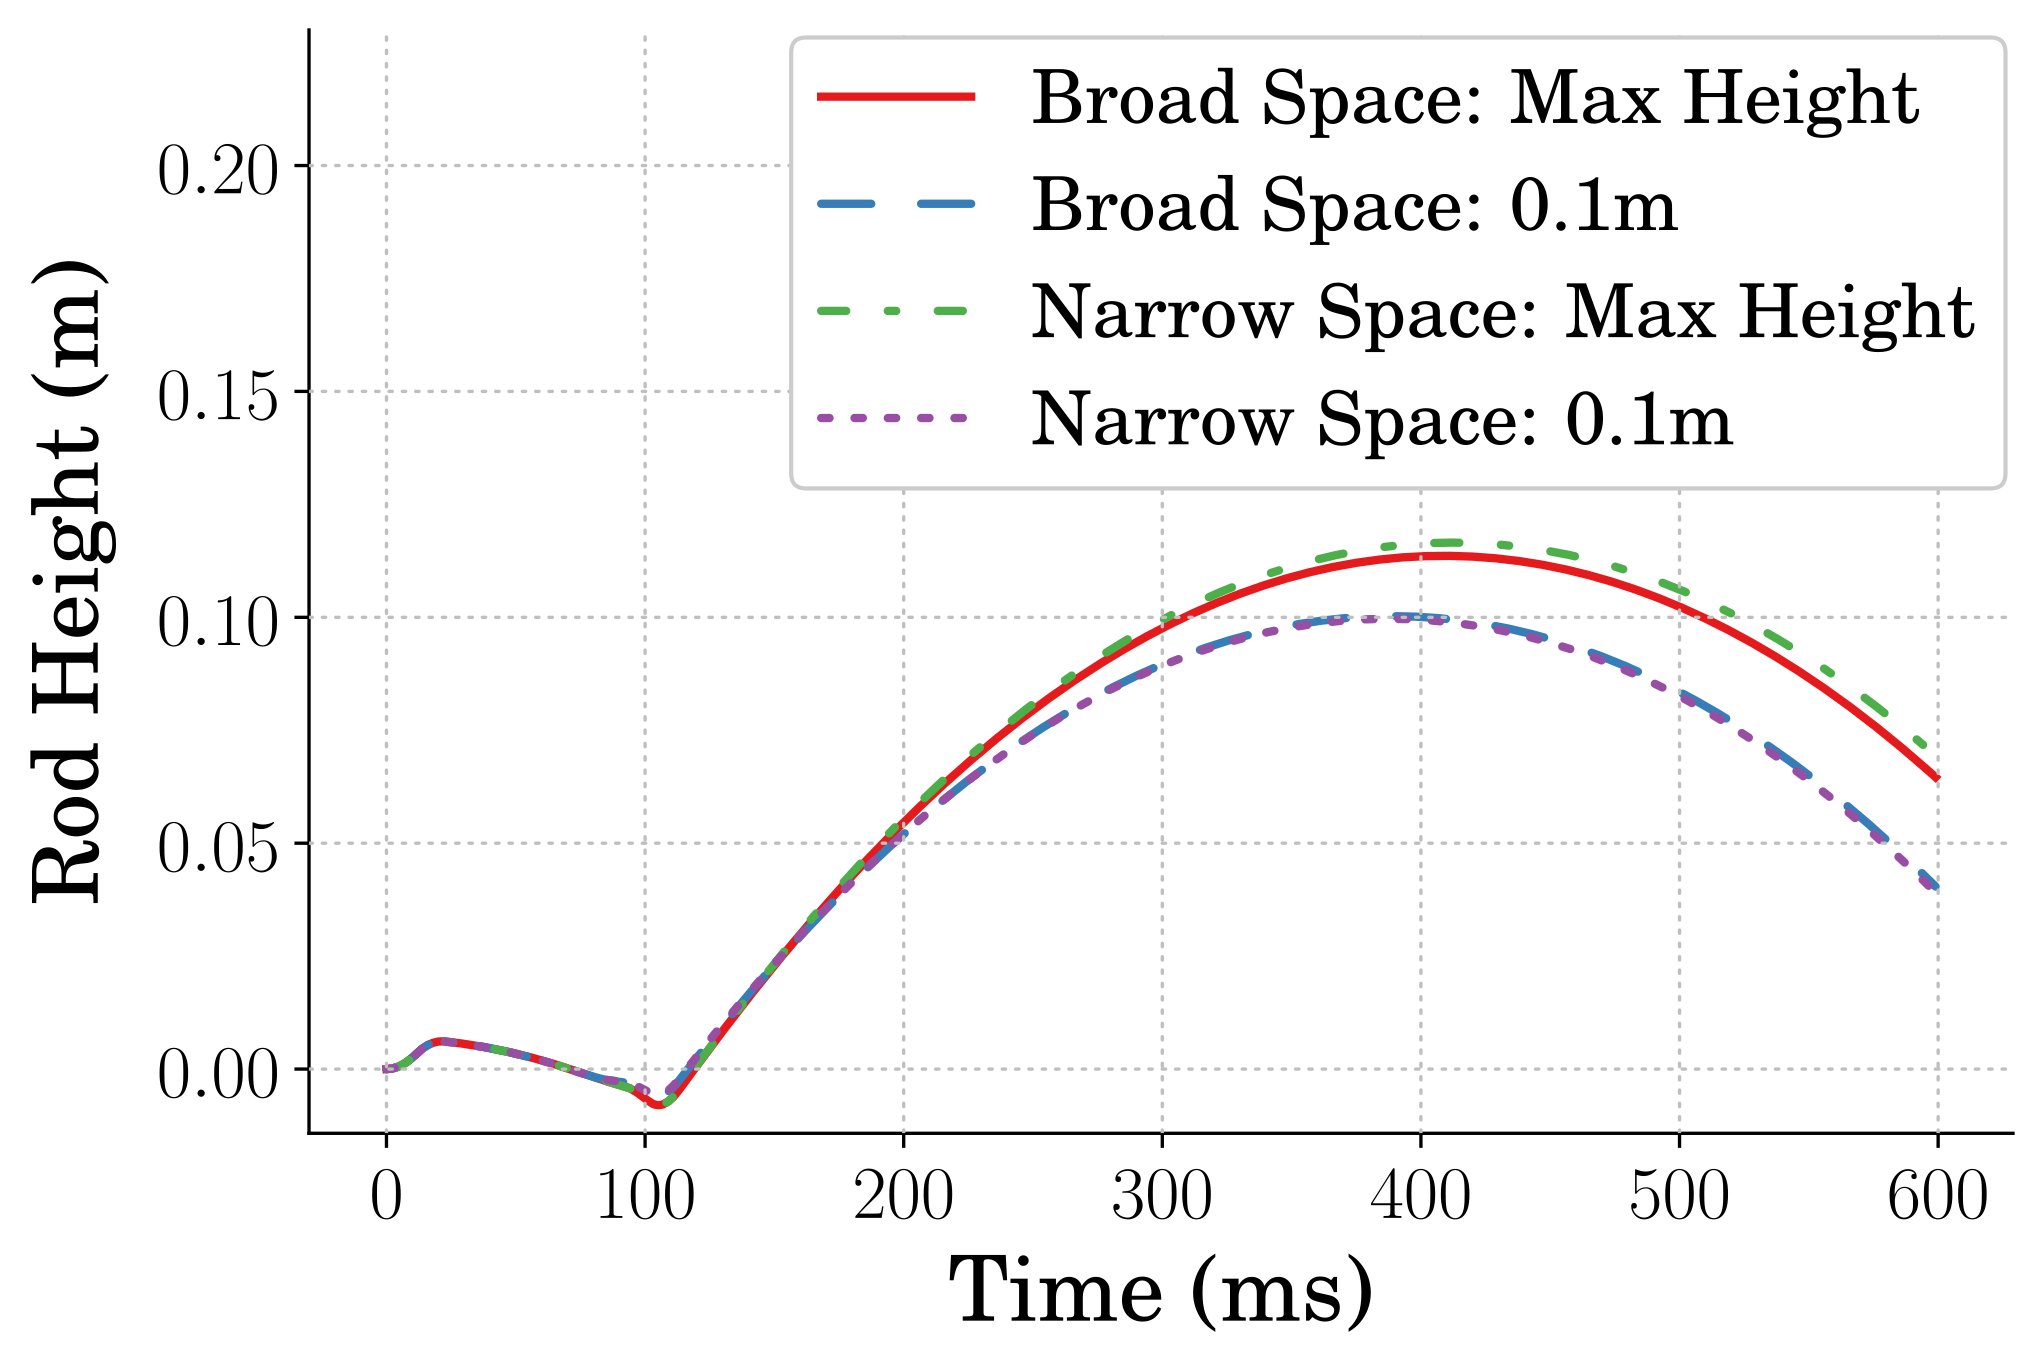
\includegraphics[width=0.75\textwidth]{figures/Ch4/timeseries/TimeseriesHeight.png}  
        \caption{Height vs Time of Average Optimal Designs}
        \label{fig:height_vs_time}
\end{figure}
% 
\begin{figure}[tb!]
        \centering
        \begin{subfigure}{0.75\textwidth}
        \centering
        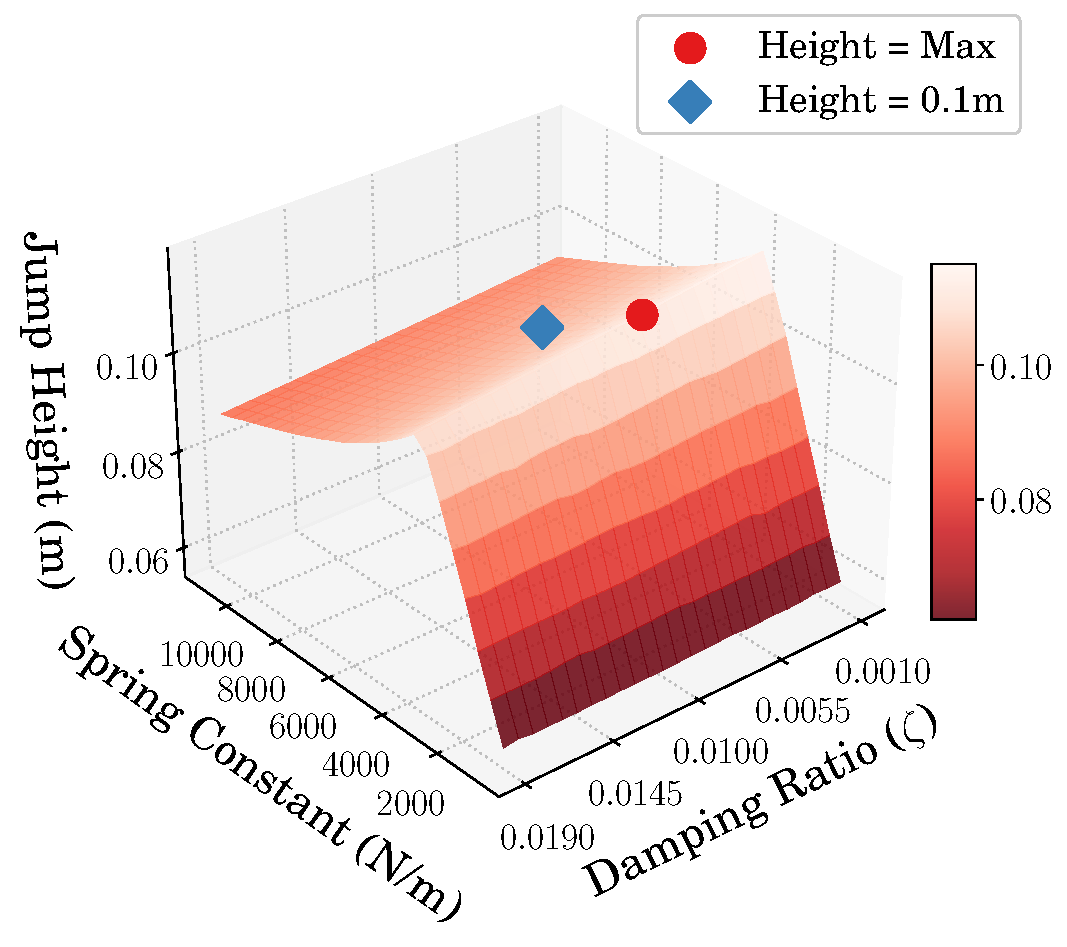
\includegraphics[width=\linewidth]{figures/Ch4/design_space_narr/3D_Plot_0.01_.pdf}
        \caption{Average Design Performance Within Narrow Design Space}
        \label{fig:des_performance_wide}
        \end{subfigure} \\
        \begin{subfigure}{0.75\textwidth}
        \centering
        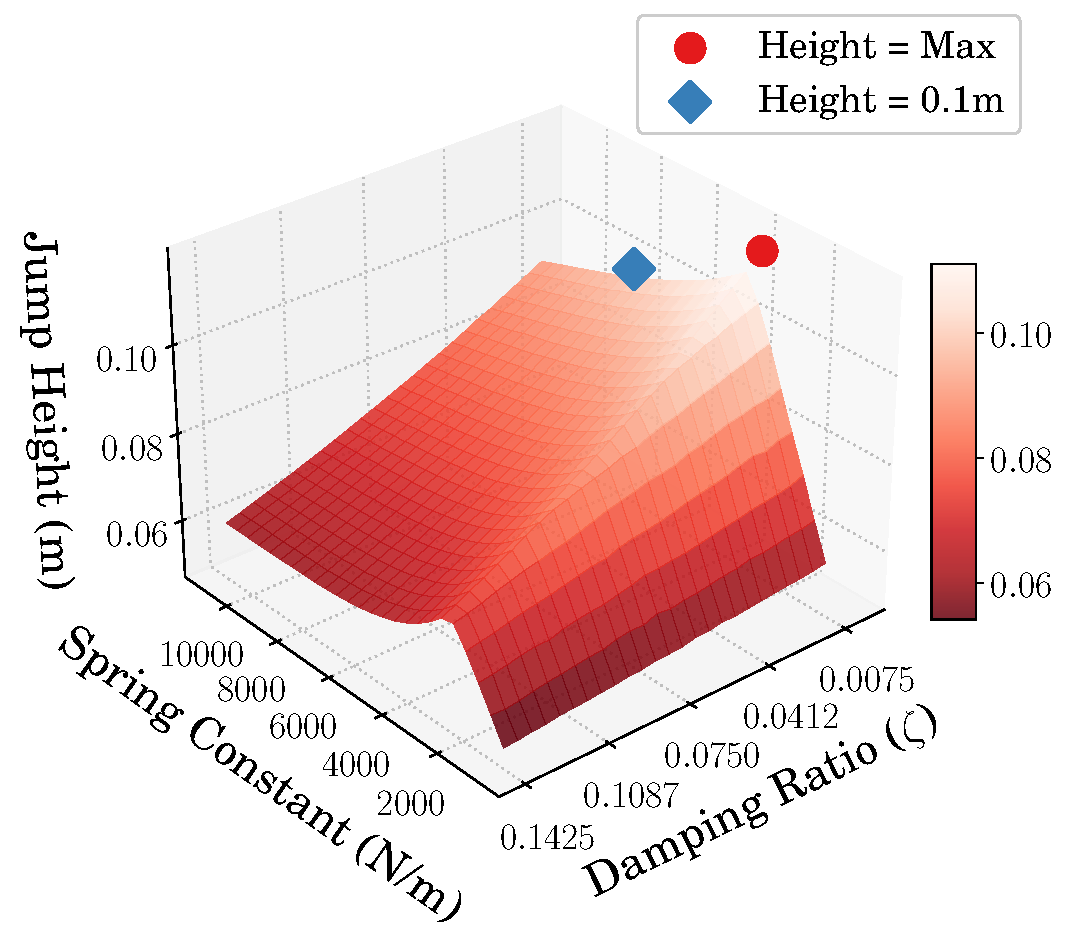
\includegraphics[width=\linewidth]{figures/Ch4/design_space_wide/3D_Plot_0.075_.pdf}
        \caption{Average Design Performance Within Wide Design Space}
        \label{fig:des_performance_narrow}
        \end{subfigure} 
         \caption{Reference Jumping Performance of the Monopode}
         \label{fig:des_performance}
\end{figure}

Additionally, Figure~\ref{fig:des_performance} shows the average designs, and their performance, against the design space performance data. It is apparent that in the case of the narrow design space, where the optimal design for maximizing height is more prominent, the design found is one that is approaching optimal performance. In the case of the wide design space, where the design that optimizes height is less prominent, it is apparent that the design found by the agent is only nearing the optimal design. In both design space cases, the design found to force the monopode to jump to the specified height was found within the higher values of the spring constant range, even though values did exist in the lower range that would satisfy the jumping condition.

\section{Conclusion}
The monopode model was used in conjunction with a predetermined control input to determine if a reinforcement learning algorithm (TD3) could be used to find optimal performing design parameters regarding jumping performance. This work was done in part to determine if reinforcement learning could be used as the mechanical design learner for an intelligent concurrent design algorithm. It was shown that when providing an agent with a design space that was smaller in size with a more prominent optimal value, the agents performed well in finding design parameters which met the performance constraints. The designs found were lower in variance as well, even in the in the case where the algorithm was tasked with finding a design for a specific performance within the range of possible performances. It was additionally shown that when provided with a larger design space, that additionally had many values closer to the optimal value, the agents still excelled at finding design parameters that performed close to optimal. The parameters found were higher in variance however, as expected, particularly in the case where a design was to be found to generate a specific performance. This was due to the number of design options that would satisfy the performance requirements. It should be concluded ultimately that utilizing an RL algorithm, such as TD3, for the mechanical design aspect of a concurrent design method, is a viable solution.